\section{Ergonomia de carregamento de peso}

Para uma pessoa de 18 a 35 anos, os limites de pesos que podem ser levantados sem causar problemas à sua saúde são 40 kg para homens e 20 kg para mulheres. Portanto em média 30 kg por pessoa. Deste modo, um objeto carregado por duas pessoas poderia pesar um máximo de 60 kg. Aplicando um fator de segurança de 30\%, o peso máximo para um objeto carregado por duas pessoas é aproximadamente 40 kg.

\section{TERMOVIDA – Caixa térmica para transporte de órgãos para transplantes}

O projeto TERMOVIDA consiste em uma caixa térmica para transporte de órgãos para transplantes com um sistema de refrigeração autônoma.

A legislação da ANVISA regulamenta como deve se dar o transporte de órgãos para transplante, as informações que devem ser coletadas que constatam o tempo de vida e a temperatura ideal a ser mantida para que os órgãos que sejam transportados em segurança por este dispositivo puderam indicar como deve ser o recipiente e quais sao os equipamentos necessário para que o mesmo funcione corretamente.

Neste projeto, é utilizada uma pastilha de efeito Peltier para a refrigeração da caixa, controlada por histerese, via um micro-controlador. O equipamento, utilizado durante o transporte em veículos, utiliza alimentação elétrica do sistema de 12V do veículo.

A estrutura da caixa é feita de material isolante térmico. Esta possui uma porta de ventilação na lateral, onde está posicionada a pastilha Peltier, e um espaço no qual um painel LCD sensível ao toque está alocado. O painel é responsável por mostrar as condições monitoradas.

\begin{figure}[H]
\centering
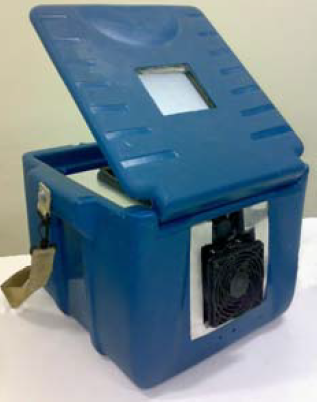
\includegraphics[scale=1]{figuras/termovida.png}
\caption{TERMOVIDA - Caixa térmica para transporte de órgãos para transplantes}
\end{figure}